% Auto-generated: clean vs poisoned trust-score distribution (pgfplots)
\begin{figure}[t]\centering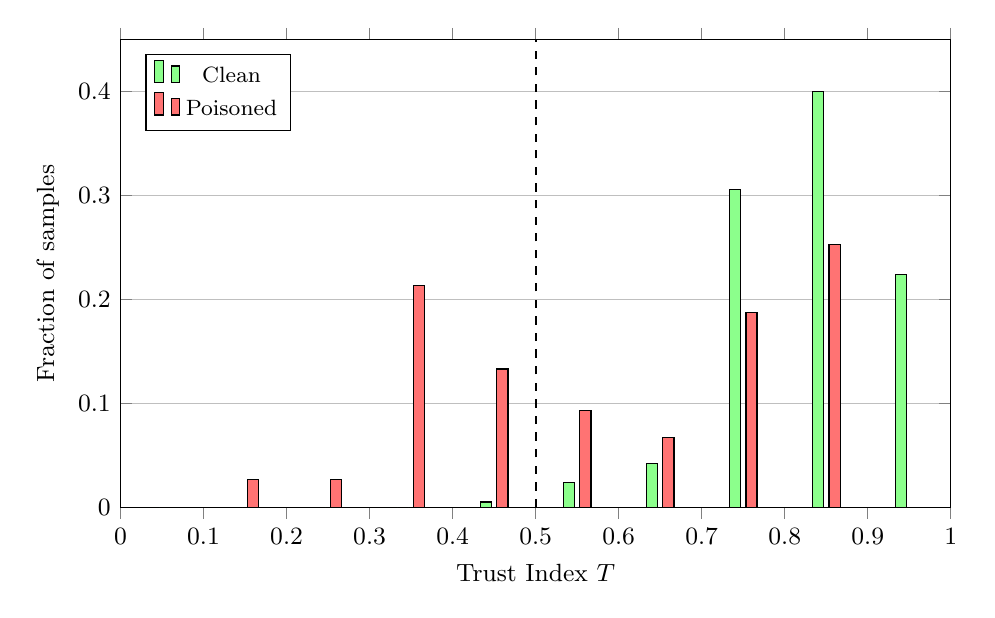
\begin{tikzpicture}
\begin{axis}[width=\columnwidth,height=0.62\columnwidth,ybar,bar width=4pt,
    xmin=0,xmax=1,ymin=0,ymax=0.45,xlabel={Trust Index $T$},ylabel={Fraction of samples},
    legend pos=north west,legend style={font=\footnotesize},ymajorgrids,font=\small]
\addplot[fill=green!45] coordinates {(0.05,0.000) (0.15,0.000) (0.25,0.000) (0.35,0.000) (0.45,0.005) (0.55,0.024) (0.65,0.042) (0.75,0.306) (0.85,0.400) (0.95,0.224)};
\addplot[fill=red!55] coordinates {(0.05,0.000) (0.15,0.027) (0.25,0.027) (0.35,0.213) (0.45,0.133) (0.55,0.093) (0.65,0.067) (0.75,0.187) (0.85,0.253) (0.95,0.000)};
\draw[dashed,thick] (axis cs:0.5,0) -- (axis cs:0.5,0.45);
\legend{Clean, Poisoned}
\end{axis}\end{tikzpicture}
\caption{Trust Index distribution for clean vs poisoned (TruthfulQA mixed, Llama~3.3~70B + MiniLM, $K{=}5$); dashed line marks the threshold $\tau{=}0.5$.}
\label{fig:trustdist}
\end{figure}